\documentclass[graybox, envcountchap]{svmult}
% Springer document settings
\usepackage[bottom]{footmisc}% places footnotes at page bottom

\usepackage{newtxtext}       % 
\usepackage[varvw]{newtxmath}       % selects Times Roman as basic font
%%%%%%%%%%%%%%%%%%%%%%%%%%%%%%%

% \usepackage{amssymb}
\usepackage{ntheorem}
\usepackage{amsmath}
\usepackage{enumitem}


\usepackage{graphicx}
\usepackage{color}
\usepackage{cite}
\usepackage{makeidx}


\usepackage{ascmac}
\usepackage{eclbkbox}
\usepackage{dsfont}

\usepackage{longtable}

\usepackage{url}

\usepackage{hyperref}

\usepackage{multicol}

%% --川口追加--
\makeatletter
\let\MYcaption\@makecaption
\makeatother
\usepackage{subcaption}
\captionsetup{compatibility=false}      % 必要に応じて

\makeatletter
\let\@makecaption\MYcaption
\makeatother
% ----

%%
\theoremstyle{plain}
\theoremheaderfont{\bfseries}
\theorembodyfont{\rmfamily}
\theoremseparator{\hspace{1ex}}
\theoremindent0cm
\theoremnumbering{arabic}
\theoremprework{\vspace{1ex}\begin{shadebox}\vspace{1ex}}
\theorempostwork{\vspace{-1ex}\end{shadebox}\vspace{1ex}}

%%
\theoremclass{theorem}

%%
\theoremclass{theorem}

%%
\theoremclass{theorem}


%%
\theoremstyle{break}
\theoremheaderfont{\bfseries}
\theorembodyfont{\rmfamily}
\theoremseparator{}
\theoremindent0cm
\theoremnumbering{arabic}
\theoremprework{\vspace{1.5ex}\begin{breakbox}\vspace{-0.5ex}}
\theorempostwork{\vspace{-0.5ex}\end{breakbox}\vspace{1.5ex}}

%%
\theoremstyle{nonumberplain}
\theoremseparator{\hspace{1ex}}

%%
\newtheorem{assumption}{Assumption}[section]

%%
\renewcommand{\theproblem}{}

\renewcommand{\theremark}{}


\newcommand{\red}[1]{{\color{red}#1}}
\newcommand{\blue}[1]{{\color{blue}#1}}
\newcommand{\green}[1]{{\color{green}#1}}

\DeclareMathOperator*{\argmax}{arg\,max}

\newcommand{\bm}[1]{\boldsymbol{#1}}
\newcommand{\sfT}{\mathsf{T}}

\newcommand{\advanced}{$^{\ddag}$}

\DeclareMathOperator{\sfsin}{\mathsf{sin}}
\DeclareMathOperator{\sfcos}{\mathsf{cos}}
\DeclareMathOperator{\sftan}{\mathsf{tan}}
\DeclareMathOperator{\sfarctan}{\mathsf{arctan}}

\DeclareMathOperator{\sfdiag}{\mathsf{diag}}
\DeclareMathOperator{\sfcol}{\mathsf{col}}
\DeclareMathOperator{\sfdet}{\mathsf{det}}
\DeclareMathOperator{\sfadj}{\mathsf{adj}}
\DeclareMathOperator{\sftrace}{\mathsf{trace}}

\DeclareMathOperator{\real}{\mathsf{Re}}

\DeclareMathOperator{\sfker}{\mathsf{ker}}
\DeclareMathOperator{\sfim}{\mathsf{im}}

\DeclareMathOperator{\sfdim}{\mathsf{dim}}
\DeclareMathOperator{\sfspan}{\mathsf{span}}

\DeclareMathOperator{\sfint}{\mathsf{int}}

\DeclareMathOperator*{\sfmin}{\mathsf{min}}
\DeclareMathOperator*{\sfmax}{\mathsf{max}}
\DeclareMathOperator*{\sfsup}{\mathsf{sup}}

\DeclareMathOperator{\sfsat}{\mathsf{sat}}

\newcommand{\mat}[1]{\left[\: \begin{matrix} #1 \end{matrix} \:\right]}
\newcommand{\spliteq}[1]{\begin{split} #1 \end{split}}
\newcommand{\simode}[1]{\begin{cases}  \begin{split} #1 \end{split} \end{cases}}

\newcommand{\proofend}{\hfill \rule{2mm}{3mm}}

\newcommand{\Xti}{X_i'}
\newcommand{\Xsi}{X_i}

\newcommand{\Xtone}{X_1'}
\newcommand{\XtN}{X_N'}

\newcommand{\Xt}{X'}
\newcommand{\Xs}{X}

\newcommand{\taudi}{\tau_i}
\newcommand{\taud}{\tau}

\newcommand{\Cgi}{b_i}


\newcommand{\Ifd}{I_{\rm field} }

\newcommand{\matlab}{\textsc{Matlab} }





%% --川口追加--
\newcommand{\thshift}{\theta_{12}}
\newcommand{\thshiftb}{\theta_{32}}
\newcommand{\Ysa}{\bm y_{12}}
\newcommand{\bca}{c_{12}}
\newcommand{\Ysb}{\bm y_{32}}
\newcommand{\bcb}{c_{32}}
\newcommand{\bcij}{c_{ij}}
\newcommand{\Is}{{\bm I}_{12}' }
\newcommand{\im}{\bm j}
\newcommand{\tr}{{\sf T}}

%%%%%%%%%%%%%%%%%%%%%%%%% code lines %%%%%%%%%%%%%%%%%%%%%%%%%%%%%%%%%%%%%%%%%%
\usepackage{listings}
\usepackage{xcolor}
\renewcommand{\lstlistingname}{Program}% Listing -> Algorithm
\renewcommand{\lstlistlistingname}{List of \lstlistingname s}% List of Listings -> List of Algorithms

\definecolor{codegreen}{rgb}{0,0.6,0}
\definecolor{codegray}{rgb}{0.5,0.5,0.5}
\definecolor{codepurple}{rgb}{0.58,0,0.82}
\definecolor{backcolour}{rgb}{0.95,0.95,0.92}

\lstdefinestyle{mystyle}{
    backgroundcolor=\color{backcolour},   
    commentstyle=\color{codegreen},
    keywordstyle=\color{magenta},
    numberstyle=\tiny\color{codegray},
    stringstyle=\color{codepurple},
    basicstyle=\ttfamily\footnotesize,
    breakatwhitespace=false,         
    breaklines=true,                 
    captionpos=b,                    
    keepspaces=true,                 
    numbers=left,                    
    numbersep=5pt,                  
    showspaces=false,                
    showstringspaces=false,
    showtabs=false,                  
    tabsize=2
}

\lstset{style=mystyle}

\begin{document}

\chapter{Numerical simulation examples of a large-scale model}\label{chap:largesim}

In this Chapter, we apply the fundamentals explained so far to perform numerical
simulations of a standard large-scale model called the IEEE 68-bus system model.
The structure of this chapter is as follows. First, in Section \ref{sec:IEEE68},
we organize the numerical data of transmission lines, loads, and generators in
the IEEE 68-bus system model. Next, in Section \ref{sec:IEEE68AGC}, we analyze
the effect of automatic generation control on load fluctuations. Specifically,
we analyze the changes in generator and bus variables when the load impedance
changes gradually over a few hours. Finally, in Section \ref{sec:IEEE68PSS}, we
analyze the transient stability of the system with respect to bus grounding. In
particular, we demonstrate that incorporating system stabilizing devices
independently designed for each generator based on retrofit control theory can
significantly improve system stability.

\section{Power system model under consideration}\label{sec:IEEE68}

\begin{figure}[t]
\centering
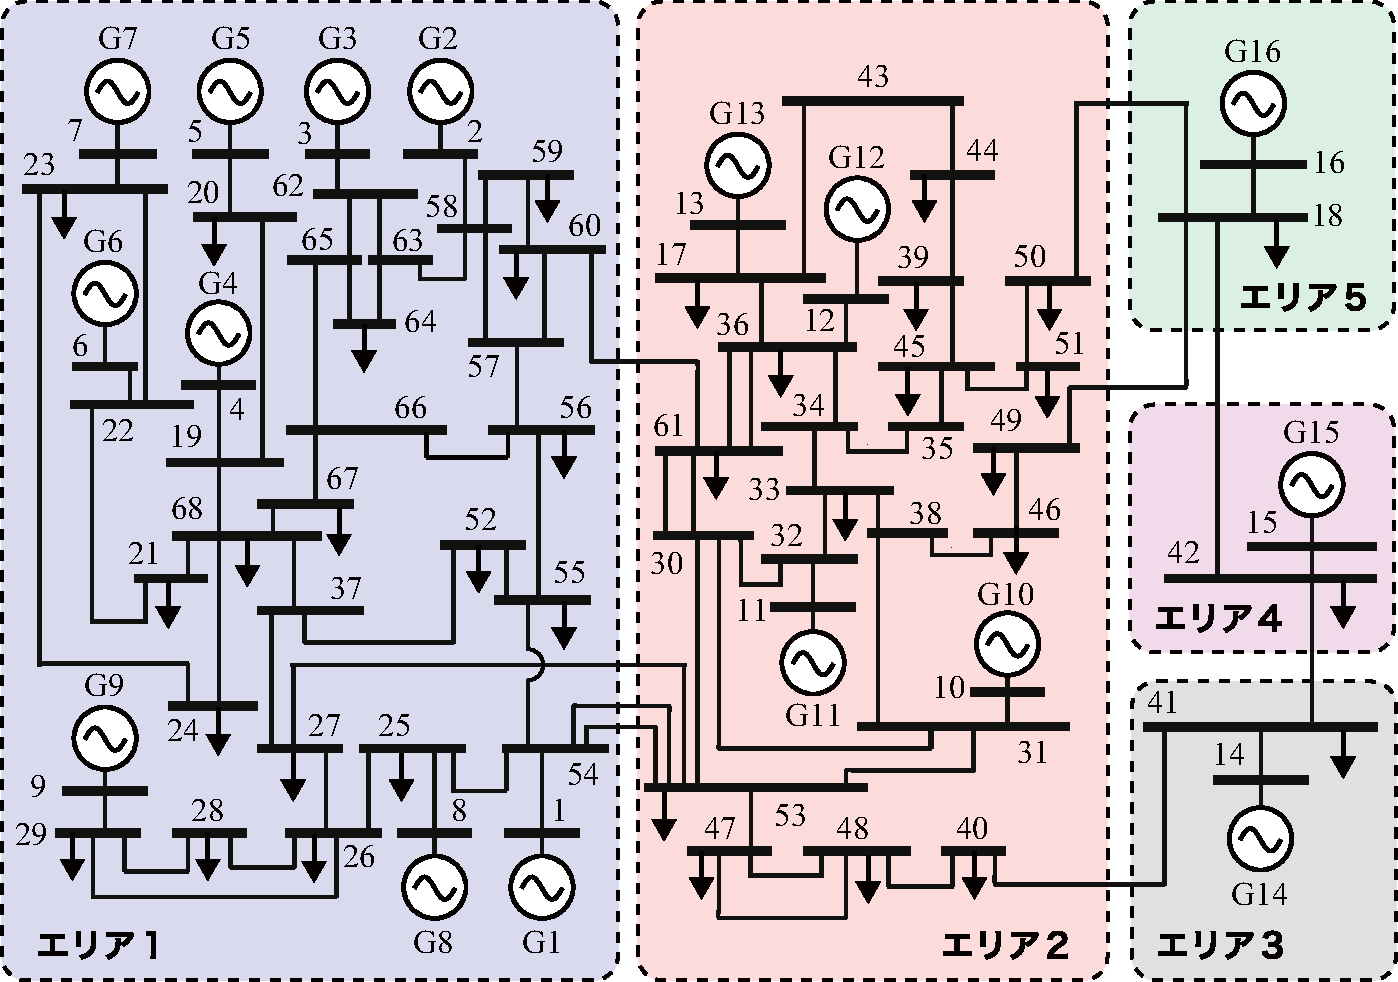
\includegraphics[width = .99\linewidth]{figs/IEEE68bus}
\medskip
\caption{\textbf{IEEE68 bus system model}}
\label{fig:IEEE68bus}
\medskip
\end{figure}

\subsection{IEEE68 bus system model}

In this section, we present numerical simulation results using the IEEE68 bus
power system model (Figure \ref{fig:IEEE68bus}). This model consists of 68
buses, with generators connected to 16 buses and loads connected to 35 buses.
The "Area 1" in Figure \ref{fig:IEEE68bus} represents the power system in the
northeastern United States, while "Area 2" represents the power system in the
state of New York. In addition, Areas 3 to 5 represent the power systems around
New York State, each represented by one set of generators and loads.

The transmission lines are modeled considering the ground capacitance as
explained in Section \ref{sec:transmodc}. The constants of each transmission
line are set to the values shown in Table \ref{table:ieee68lines}. The first
column shows the bus numbers at both ends of the transmission line, and the
second, third, and fourth columns show the resistance, reactance, and ground
capacitance values of the transmission line, respectively. These are standard
values shown in \cite[Appendix A]{pal2006robust}. Furthermore, we use the
salient-pole generator model explained in Section \ref{sec:genmodadv} for the
generators.  The constants for each generator are set to the values shown in
Table \ref{table:ieee68genpara}, which are also shown in the aforementioned
literature.

\subsection{Data sheet for power flow calculation}

The data sheets for the generator buses used in power flow calculations are
shown in Table \ref{table:ieee68datag}. Similarly, the data sheet for the load
buses is shown in Table \ref{table:ieee68datal}. These values are also cited
from \cite[Appendix A]{pal2006robust}.

\subsection{Load model}

The constant impedance load model described in Section \ref{sec:loadpr} is
adopted for the load model. The impedance values of the loads determined from
the power flow calculation results for the data sheets in Table
\ref{table:ieee68datag} and Table \ref{table:ieee68datal} are shown in Table
\ref{table:ieee68loads}. Note that bus 16 is set as the slack bus, and the value
of $P_{16}^{\star}$ is calculated as 33.68.

\section{Frequency stability analysis for load fluctuations}\label{sec:IEEE68AGC}

\subsection{Load fluctuation settings}

In this section, we observe the time response of the angular frequency deviation
when the impedance values of the loads are changed. The impedance values of the
loads are increased linearly by 10\% per hour based on the values in
Table \ref{table:ieee68loads}. That is, the impedance of each load is set as:

\begin{equation}\label{eq:loadvary68}
  z_{{\rm load}i}(t) = \left(1+\tfrac{1}{36000}t \right) \left( r_{{\rm load}i} + \bm{j} x_{{\rm load}i} \right)
\end{equation}
where $t$ is the time in [s].

\subsection{When the machine input and field input of the generator are constant}\label{sec:constPV}

Consider the case where both the mechanical and excitation inputs to the
generator, which are external inputs, are constant. From the steady-state power
flow solution given in the data sheets of Table \ref{table:ieee68datag} and
Table \ref{table:ieee68datal}, the time response of the frequency deviation for
all generators is shown in Figure \ref{fig:omegasAGC}(a) when the impedance of
the load changes according to Equation \ref{eq:loadvary68}. In this case, since
the load disturbance causes an imbalance in supply and demand, the frequency
deviation does not converge to zero. Moreover, due to the increase in power
consumption as the impedance of the load increases, the frequency deviation
initially increases in the negative direction for about 7 seconds, and then
diverges in the positive direction as the power system model becomes unstable.

\begin{figure}[t]
  \centering
  {
  \begin{minipage}{0.49\linewidth}
    \centering
    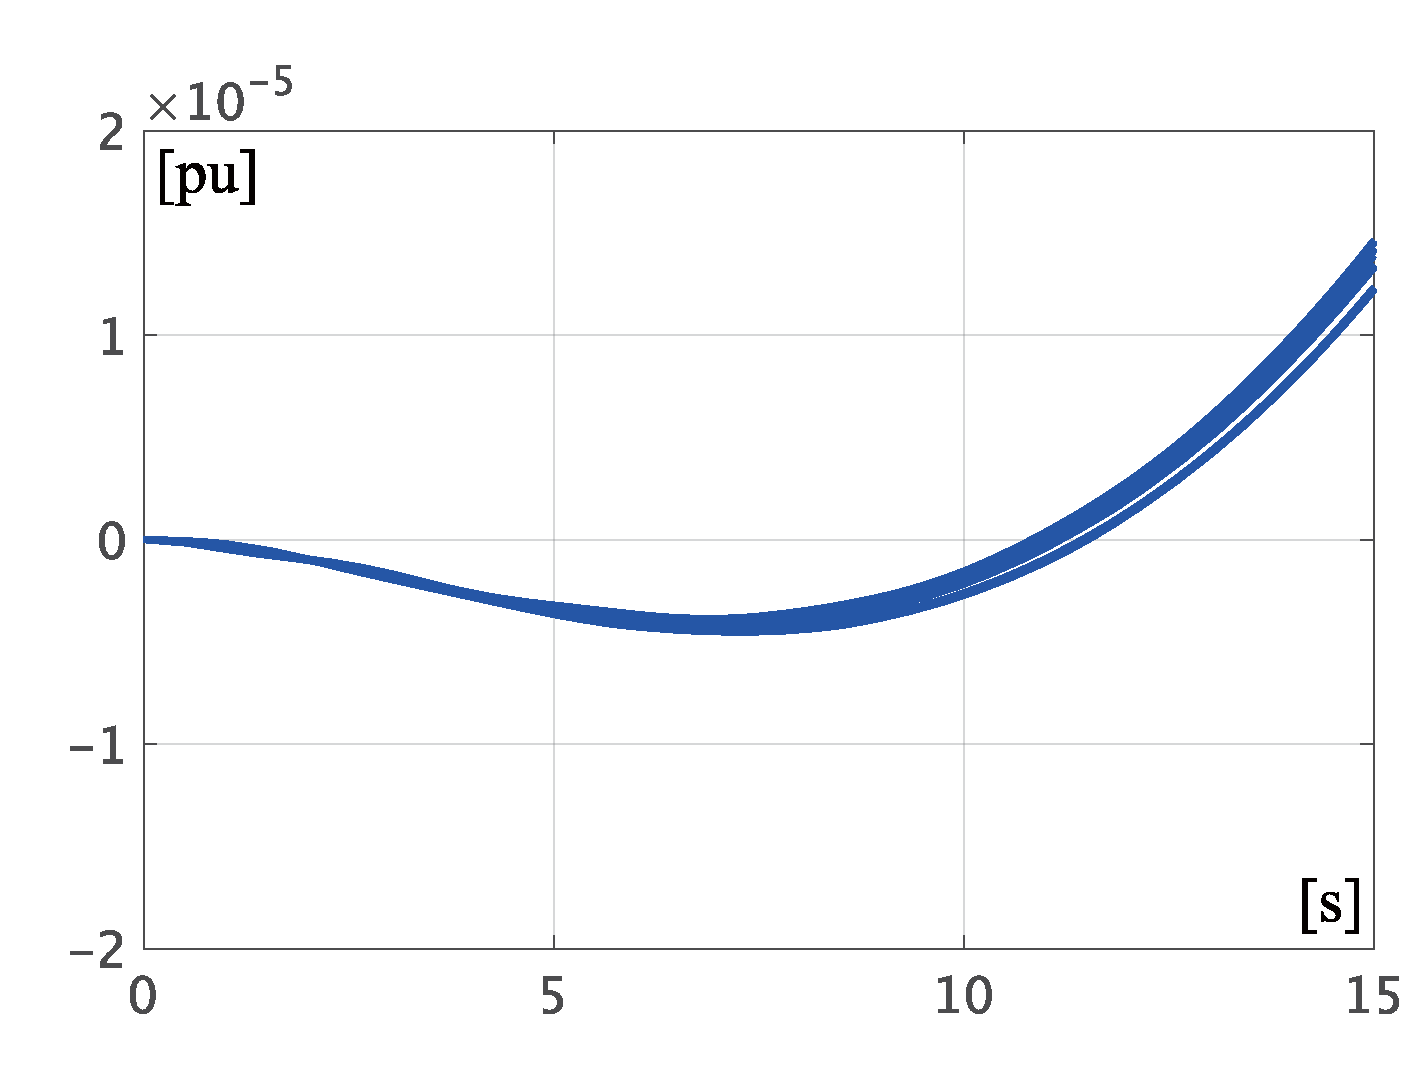
\includegraphics[width = 1.0\linewidth]{figs/WOavrWOagc}
    \subcaption{Case where mechanical input and excitation input of the generator are constant}
    \medskip
  \end{minipage}
  \begin{minipage}{0.49\linewidth}
    \centering
    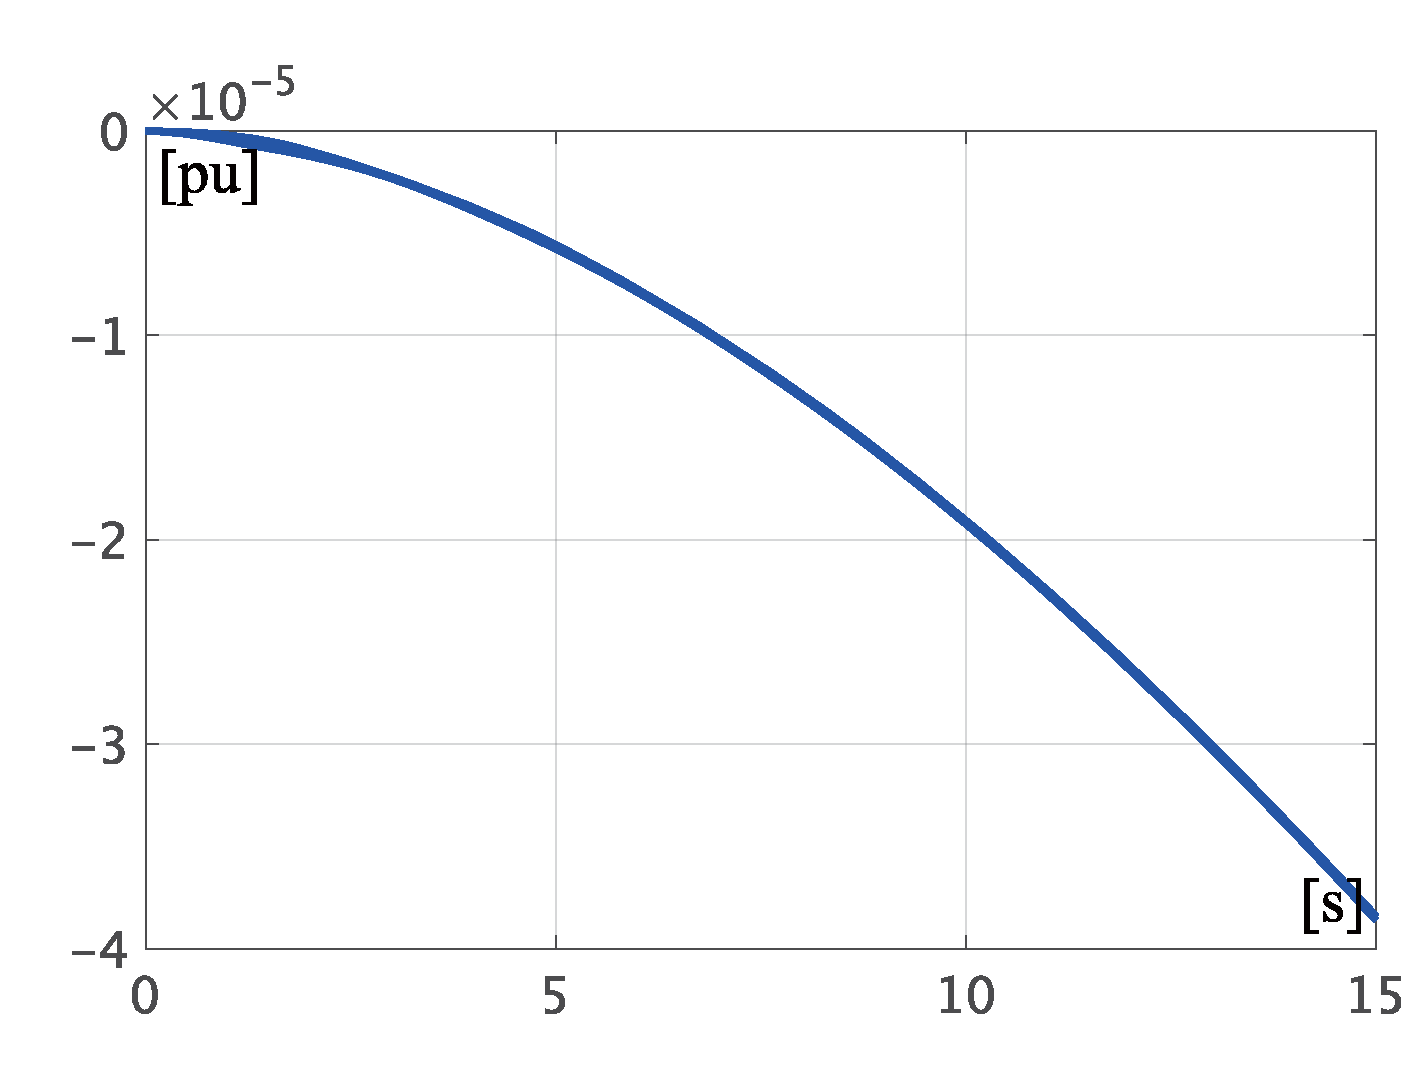
\includegraphics[width = 1.0\linewidth]{figs/WavrWOagc}
    \subcaption{Case where mechanical input of the generator is constant}
    \medskip
  \end{minipage}
 \begin{minipage}{0.49\linewidth}
    \centering
    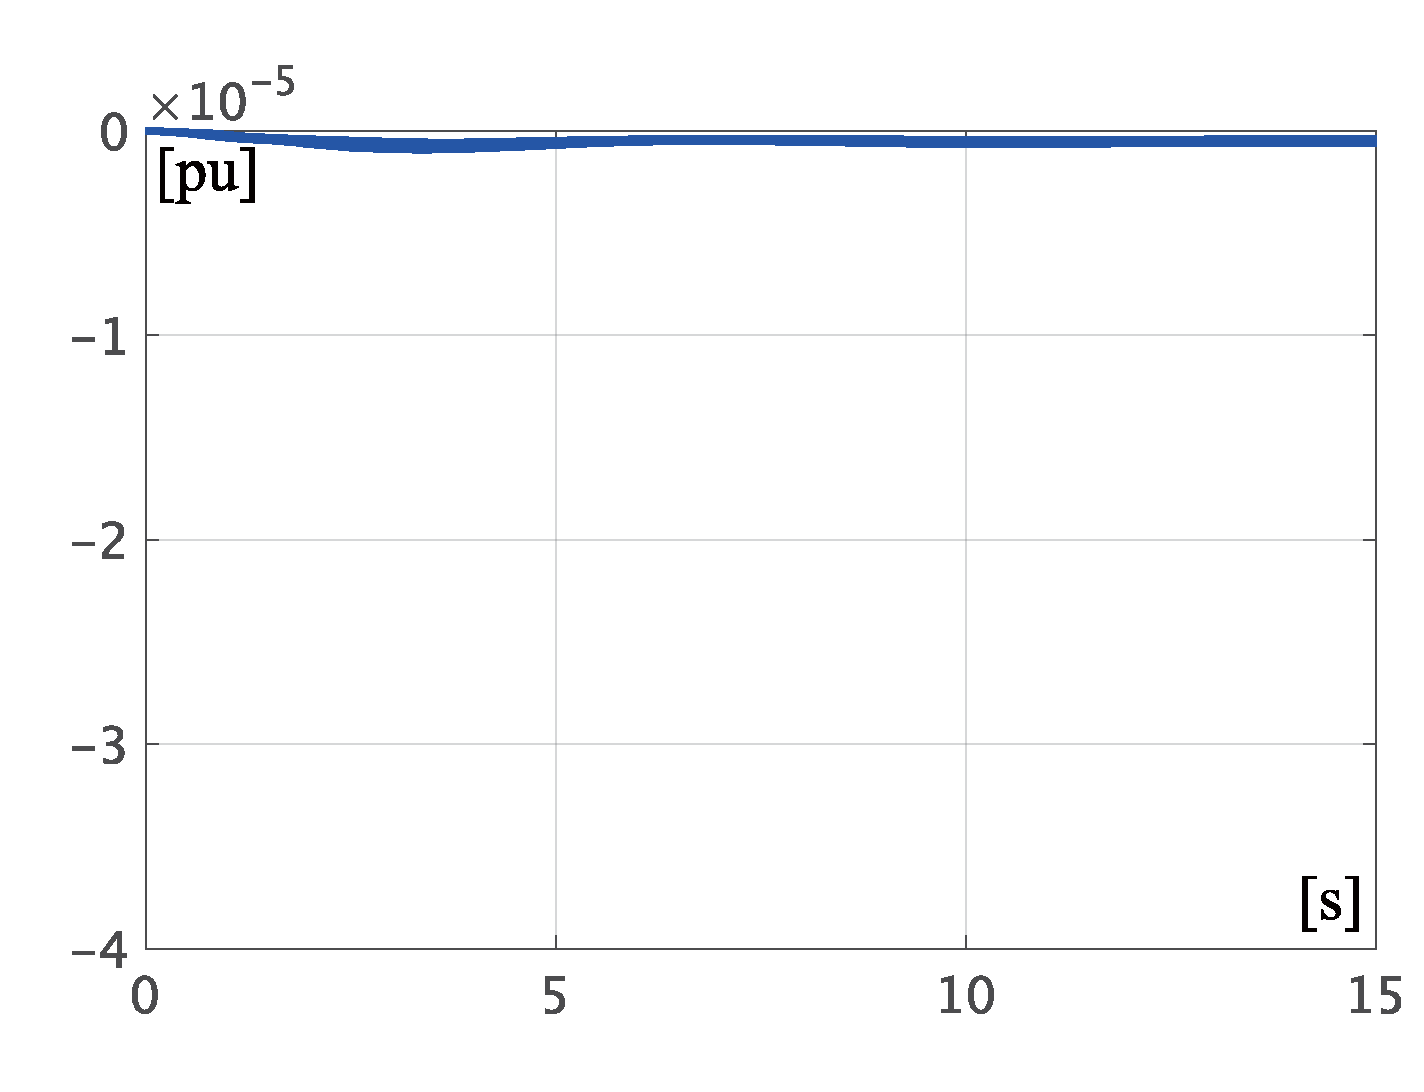
\includegraphics[width = 1.0\linewidth]{figs/WavrWagc}
    \subcaption{Case where mechanical input of the generator is controlled}
    \medskip
  \end{minipage}
  \begin{minipage}{0.49\linewidth}
    \centering
    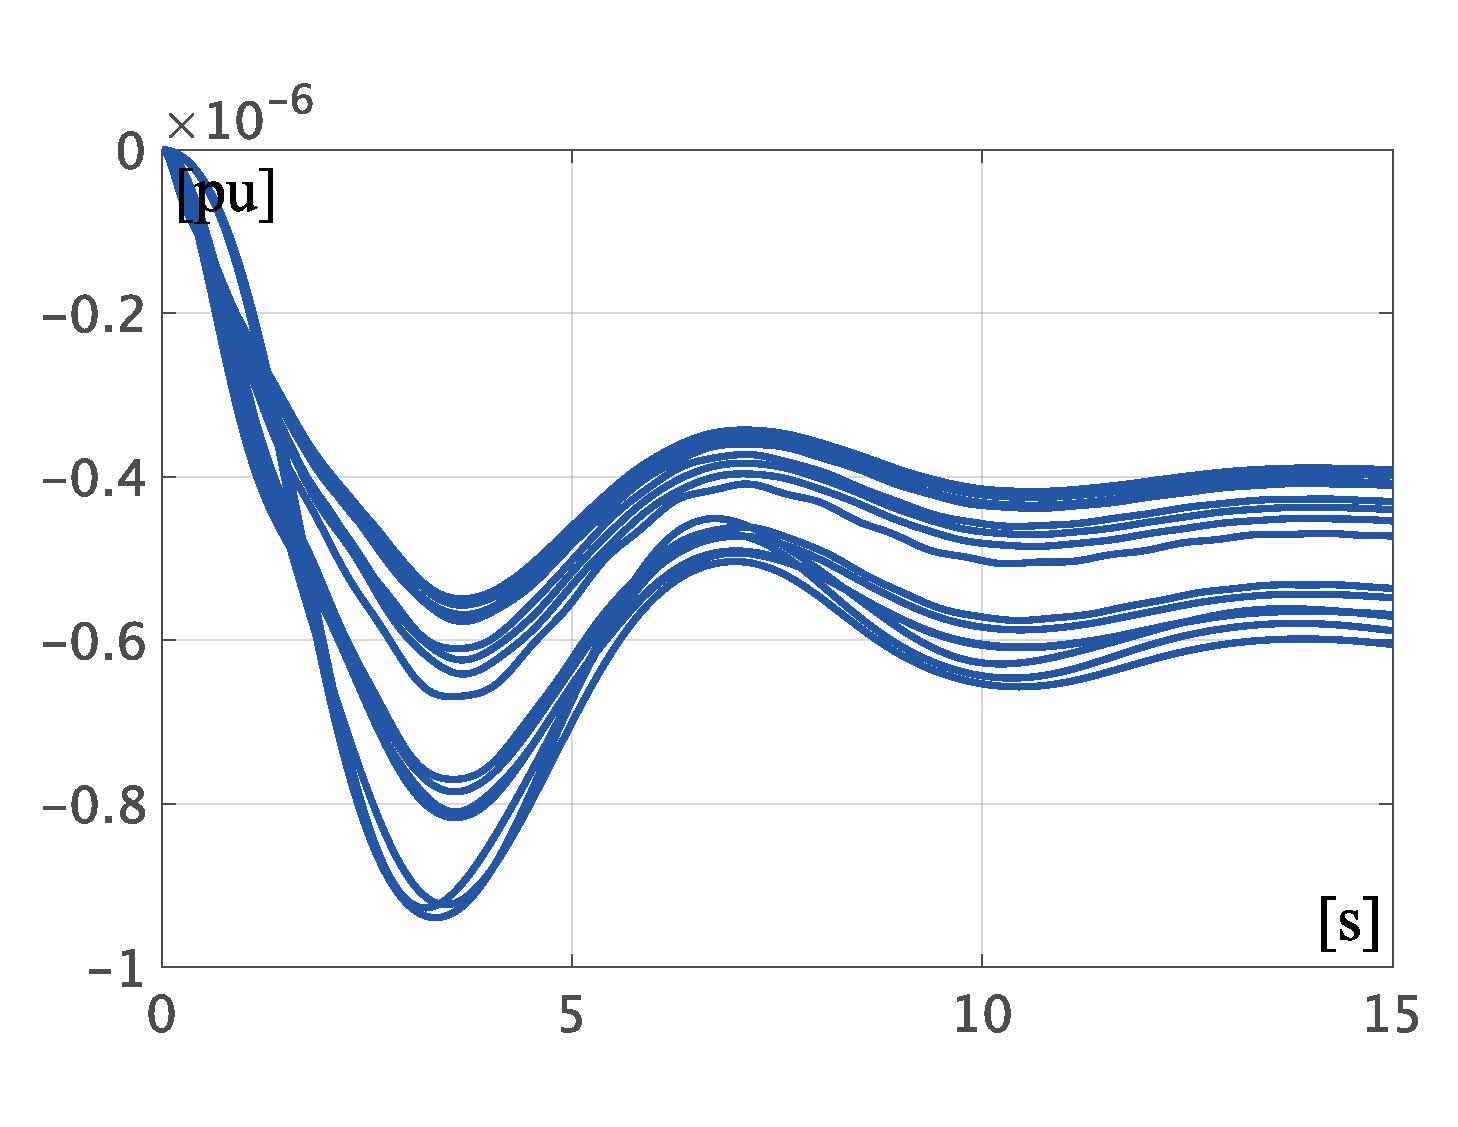
\includegraphics[width = 1.0\linewidth]{figs/WavrWagcL}
    \subcaption{Case where mechanical input of the generator is controlled (zoomed in)}
    \medskip
  \end{minipage}
  }
  \medskip
  \caption{\textbf{Time response of angular frequency deviation to load variation}}
  \label{fig:omegasAGC}
\medskip
\end{figure}

\subsection{Case where the Mechanical Input is Constant}\label{sec:onlyAVR}

Consider the case where an automatic voltage regulator that controls the
excitation input of the generator and a power system stabilizer are installed in
all generators. The automatic voltage regulator is set to the IEEE ST1 model
described in Section \ref{sec:avrov}.  Specifically, for all generator buses
$i$, it is set to:

\begin{equation*}
  \begin{aligned}
    0.015 \dot{V}_{{\rm tr}i} & = - V_{{\rm tr} i} +  |\bm{V}_i|  \\
    V_{{\rm field}i} &= 20 ( V_{{\rm ref}i}^{\star} + V_{{\rm pss}i}- V_{{\rm tr}i} )
  \end{aligned}
\end{equation*}

In addition, the power system stabilizer is set to the IEEE PSS1 model described
in Section \ref{sec:pssintro}. Specifically, for all generator buses $i$, it is
set to:

\begin{equation*}
  \begin{aligned}
    1.4 \dot{\xi}_{{\rm ws}i} &=
    - \xi_{{\rm ws}i}
    + 9.5 \Delta \omega_i \\
    v_{{\rm ws}i} &= 9.5 \Delta \omega_i - \xi_{{\rm ws}i}
  \end{aligned}
  \begin{aligned}
    0.033 \dot{\xi}_{i} &=
    - \xi_{i}
    + 0.79 %\tfrac{ 0.033 }{ 0.154 }
    v_{{\rm ws}i} \\
    V_{{\rm pss}i} &= 4.67 ( v_{{\rm ws}i} - \xi_{i} )
  \end{aligned}
\end{equation*}

The time response of the frequency deviation in this case is shown in Figure
\ref{fig:omegasAGC}(b). Similar to Figure \ref{fig:omegasAGC}(a), it can be seen
that due to load fluctuations, the supply-demand balance is not satisfied, and
the frequency deviation does not become zero.  Note that the mechanical input of
the generator is also set to be constant for all generators, as described in
Section \ref{sec:constPV}.

\subsection{Case where machine input is controlled by an automatic generation controller}

Consider incorporating an automatic generator control to control the mechanical
input of a generator. Here, for each area in Figure \ref{fig:IEEE68bus}, we will
incorporate the broadcast-type PI controller explained in Section
\ref{sec:broadPI}. Specifically, let $\mathcal{I}^{(l)}_{\rm G}$ denote the
index set of generator buses in area $l$. Then, for the automatic generator
control in area $l$, we set:

\begin{equation*}
  \begin{aligned}
    \dot{\xi}^{(l)}&=  \Delta \omega_{\rm ave}^{(l)}\\
    P_{{\rm mech}i} &= P_{i}^{\star} 
    - \tfrac{ P_{i}^{\star} }{ P_{{\rm ave}}^{{\star}} } \left(  100 \Delta \omega_{\rm ave}^{(l)} +  500  \xi^{(l)} \right),
    \qquad i \in \mathcal{I}^{(l)}_{\rm G}
  \end{aligned}
\end{equation*}
where we define the average of the deviation of angular frequency and the
average of the active power in steady-state for the generators in area $l$ as
follows:

\[
  \Delta \omega_{\rm ave}^{(l)}(t) := 
  \frac{ 1 }{|\mathcal{I}^{(l)}_{\rm G}|}
  \sum_{i \in \mathcal{I}^{(l)}_{\rm G}}  \Delta \omega_{i}(t)
  ,\qquad
  P_{{\rm ave}}^{{\star}} := 
  \frac{ 1 }{ 16 }
  \sum_{i =1}^{16}  P_{i}^{\star}
\]

It is assumed that each generator is equipped with an automatic voltage
regulator as explained in Section \ref{sec:onlyAVR}.

The time response of the frequency deviation in this case is shown in Figure
\ref{fig:omegasAGC}(c). Note that Figure \ref{fig:omegasAGC}(d) is an enlarged
version of the y-axis scale. As a result of the automatic generation control, it
can be seen that the frequency deviation is maintained around 0. Although the
impedance value of the load continues to change, the frequency deviation does
not become exactly 0, but remains at a small value of about $-1\times 10^{-6}$
[pu].

\begin{figure}[t!]
  \centering
  {
  \begin{minipage}{0.49\linewidth}
    \centering
    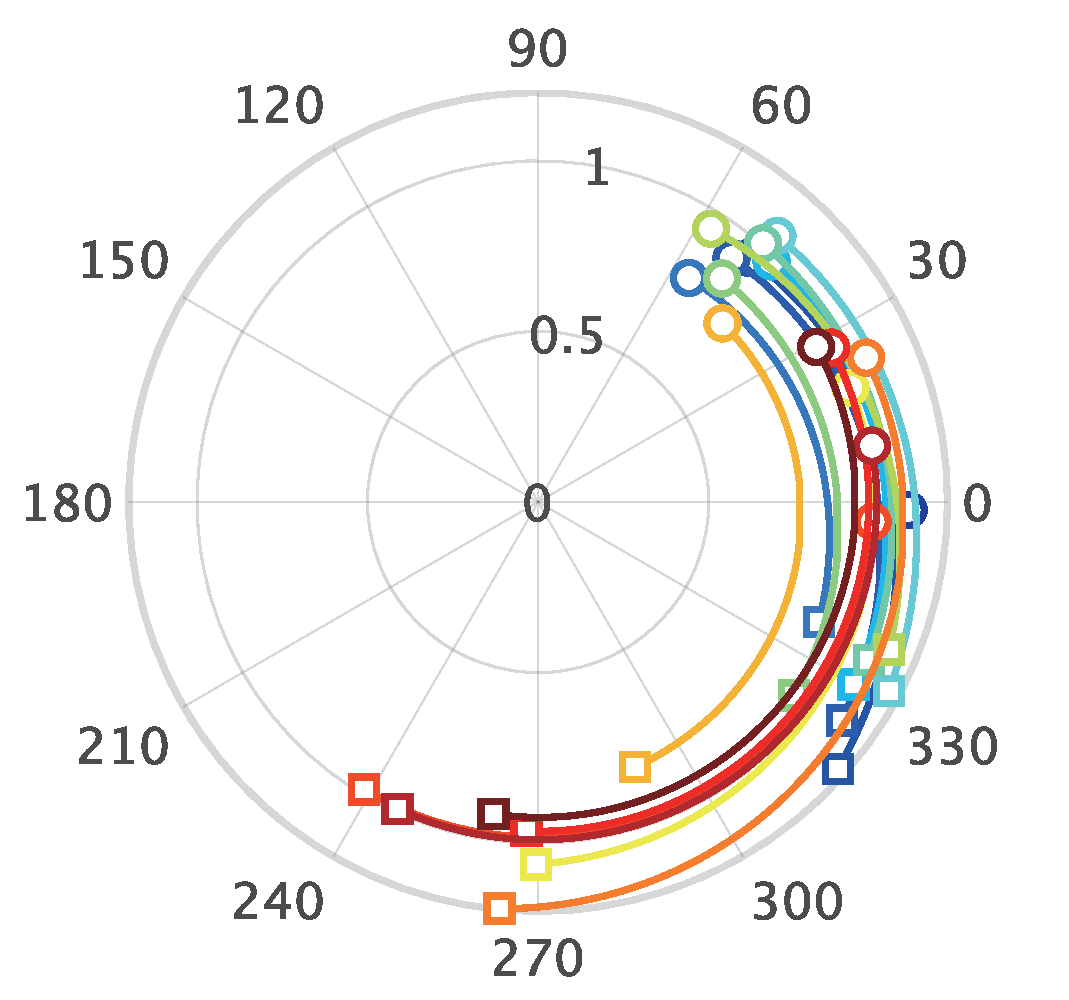
\includegraphics[width = 0.9\linewidth]{figs/Epolar}
    \subcaption{ $E_i e^{\bm{j} \delta_i}$~[pu]}
    \medskip
  \end{minipage}
  \begin{minipage}{0.49\linewidth}
    \centering
    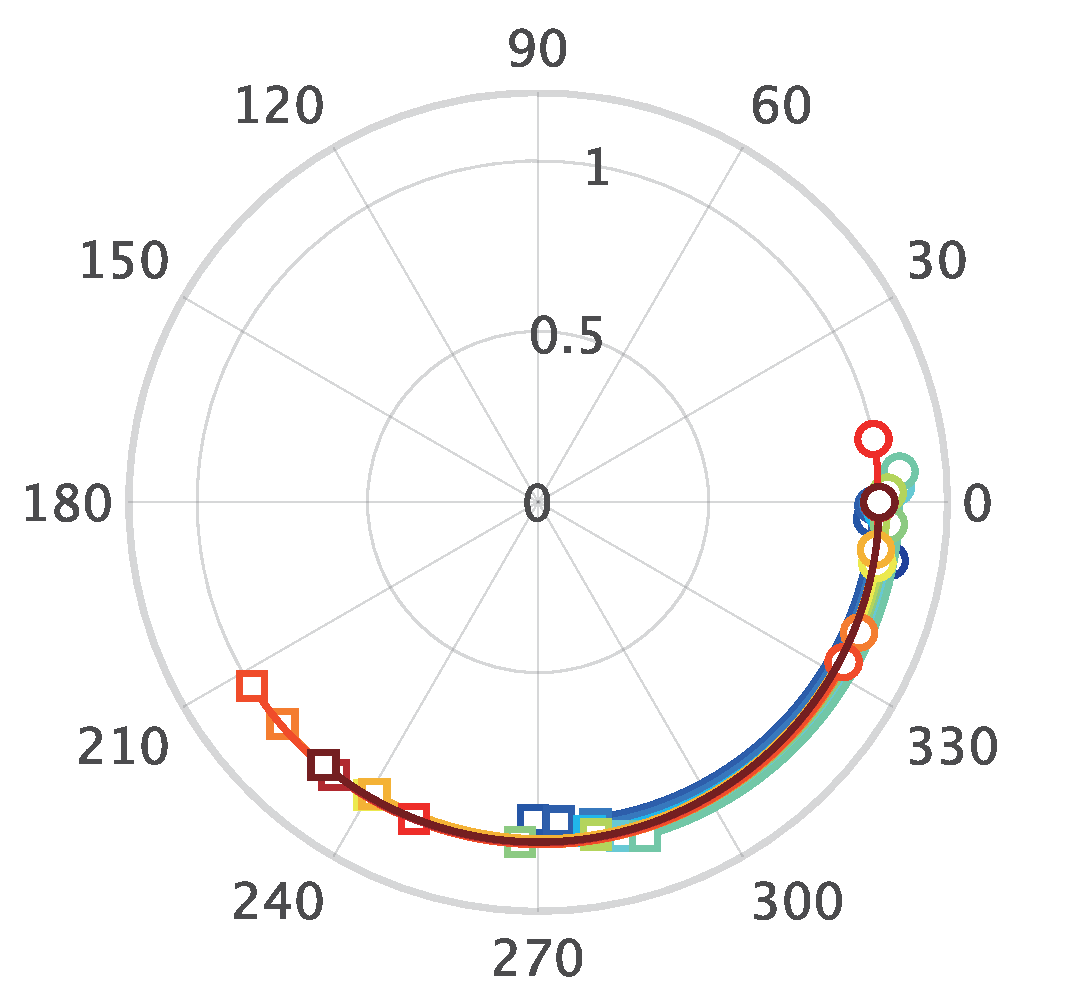
\includegraphics[width = 0.9\linewidth]{figs/Vpolar}
    \subcaption{ $\bm{V}_i$~[pu] }
    \medskip
  \end{minipage}
 \begin{minipage}{0.49\linewidth}
    \centering
    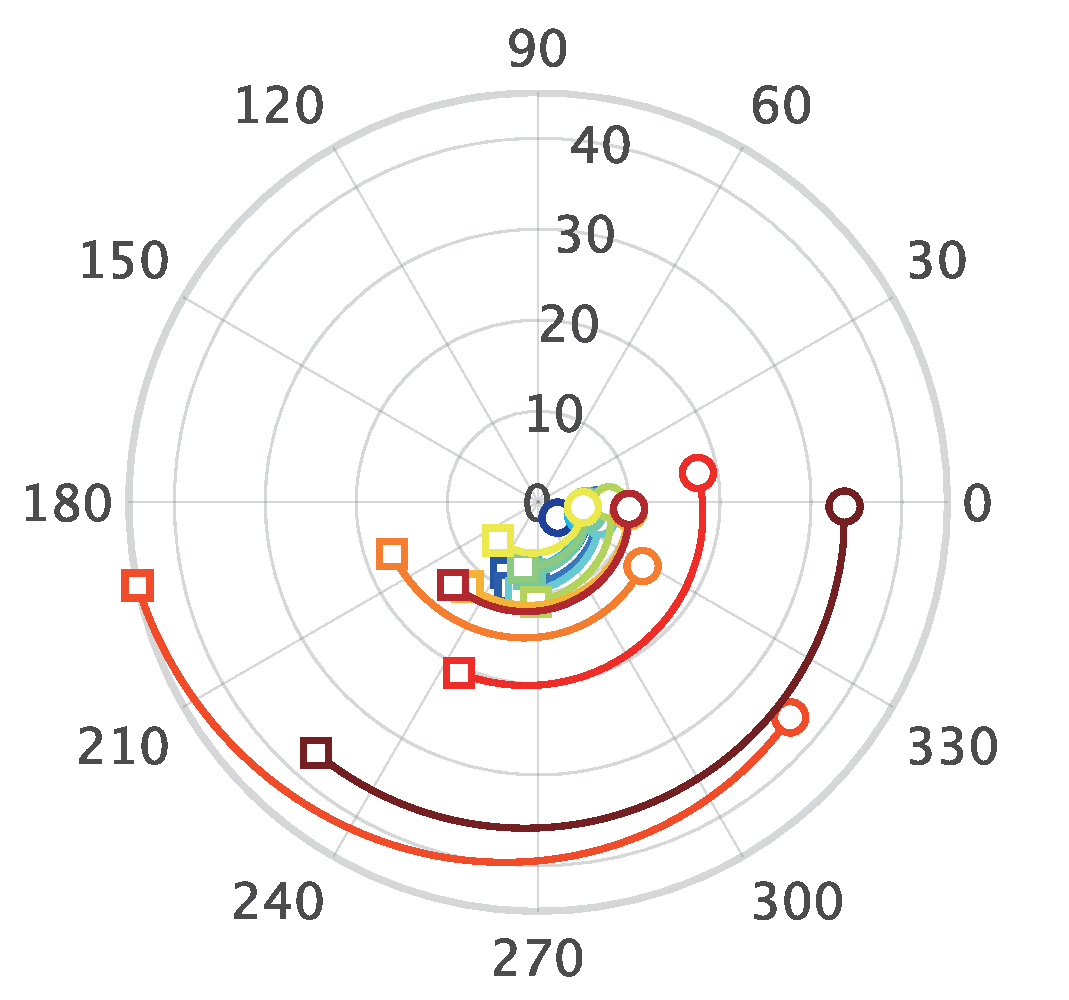
\includegraphics[width = 0.9\linewidth]{figs/Ipolar}
    \subcaption{ $\bm{I}_i$~[pu] }
    \medskip
  \end{minipage}
  \begin{minipage}{0.49\linewidth}
    \centering
    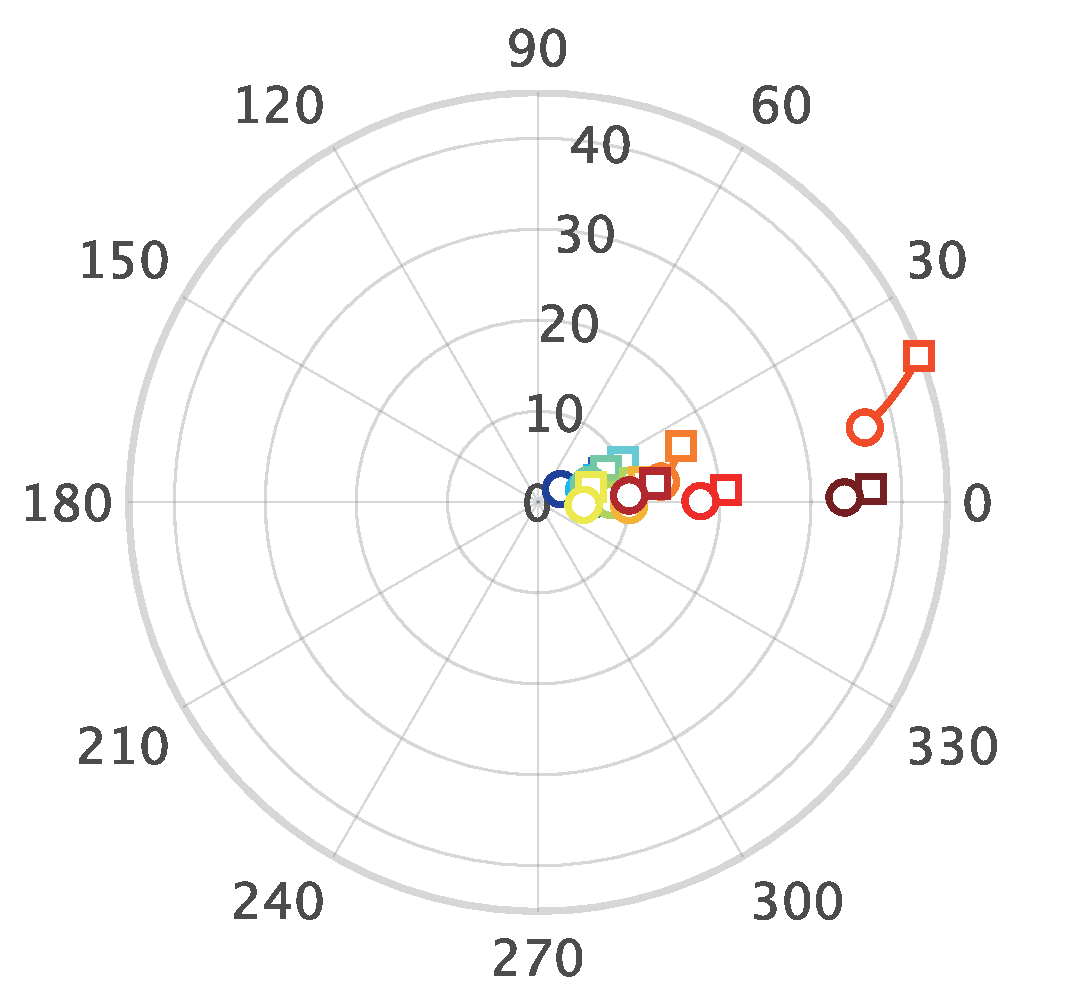
\includegraphics[width = 0.9\linewidth]{figs/PQpolar}
    \subcaption{ $P+\bm{j}Q$~[pu] }
    \medskip
  \end{minipage}
  }
  \medskip
  \caption{\textbf{Changes in generator and bus variables due to load variations.  }
  \\  \centering(Circle: initial time, square: end time)}
  \label{fig:polars}
\medskip
\end{figure}

Next, the changes in generator variables and bus variables from the initial time
to 3 hours later are shown in Figure \ref{fig:polars}. Figures
\ref{fig:polars}(a)-(d) represent the changes in $E_ie^{\bm{j}\delta_i}$,
$\bm{V}_i$, $\bm{I}_i$, and $P_i+\bm{j}Q_i$, respectively, on a polar coordinate
plane. The circle marks indicate the values at the initial time $t=0$, and the
square marks indicate the values at the final time $t=10800$. The following can
be observed from this figure:

\begin{itemize}
  \item Figure \ref{fig:polars}(a):The internal voltage of all generators is
  maintained at around 0.7 to 1.5 [pu], and the rotor angle changes gradually in
  a clockwise direction.
  \item Figure \ref{fig:polars}(b):The absolute value of the bus voltage is
  maintained around 1 [pu], and its phase changes gradually in a clockwise
  direction like the rotor angle.
  \item Figure \ref{fig:polars}(c):The absolute value of the bus current
  increases as the consumption power increases with the increase in the
  impedance value of the load.
  \item Figure \ref{fig:polars}(d):As the impedance value of the load increases,
  the supplied active power and reactive power to the bus increase.
\end{itemize}

From these results, it can be seen that frequency stabilization is appropriately
achieved by automatic generation control. In addition, for gradual load changes,
it can be seen that the internal state of the generators changes gradually
without oscillation, i.e., the entire power system is in a quasi-steady state.

\section{Transient stability analysis for bus ground faults}\label{sec:IEEE68PSS}

\subsection{Setting of ground fault}

In this section, we conduct a transient stability analysis of bus grounding.
The transient stability of a power system is evaluated as follows: Let $\Delta
\omega_i^{(k)}$ denote the angular frequency deviation of generator $i$ at bus
$k$ caused by a ground fault. Then, the sensitivity of the angular frequency
deviation of the entire power system to the grounding of bus $k$ is evaluated by
the $\mathcal{L}_2$-norm of $\Delta \omega^{(k)}$, where $\Delta \omega^{(k)}$
is a vector consisting of the angular frequency deviations $\Delta
\omega_1^{(k)},\ldots,\Delta \omega_{16}^{(k)}$ of all generators at bus $k$.
Furthermore, we define the sets of $\|\Delta \omega^{(k)}\|_{\mathcal{L}2}$ for
all generator buses and load buses, respectively, as

\begin{equation*}%\label{eq:JGJL}
  \mathcal{J}_{\rm G}:=
  \left\{
  \| \Delta \omega^{(k)} \|_{\mathcal{L}_2}
  \right\}_{k\in \{1,\ldots,16\} }
  ,\qquad
  \mathcal{J}_{\rm L}
  :=
  \left\{
  \| \Delta \omega^{(k)} \|_{\mathcal{L}_2}
  \right\}_{k\in \{17,\ldots,68\} }
\end{equation*}

Considering that a ground fault can occur at any bus, not just a specific bus,
the transient stability of bus grounding can be evaluated by considering the
smallness of the data sets $\mathcal{J}_{\rm G}$ and $\mathcal{J}_{\rm L}$ in an
appropriate sense. In this section, we use the maximum value, minimum value, and
quartiles of $\mathcal{J}_{\rm G}$ and $\mathcal{J}_{\rm L}$ shown in box plots
to compare the transient stability, in order to visualize the size of the data
dispersion. Note that the duration of the ground fault is set to 70~[ms] for all
buses.

\begin{figure}[t!]
  \centering
  {
  \begin{minipage}{0.49\linewidth}
    \centering
    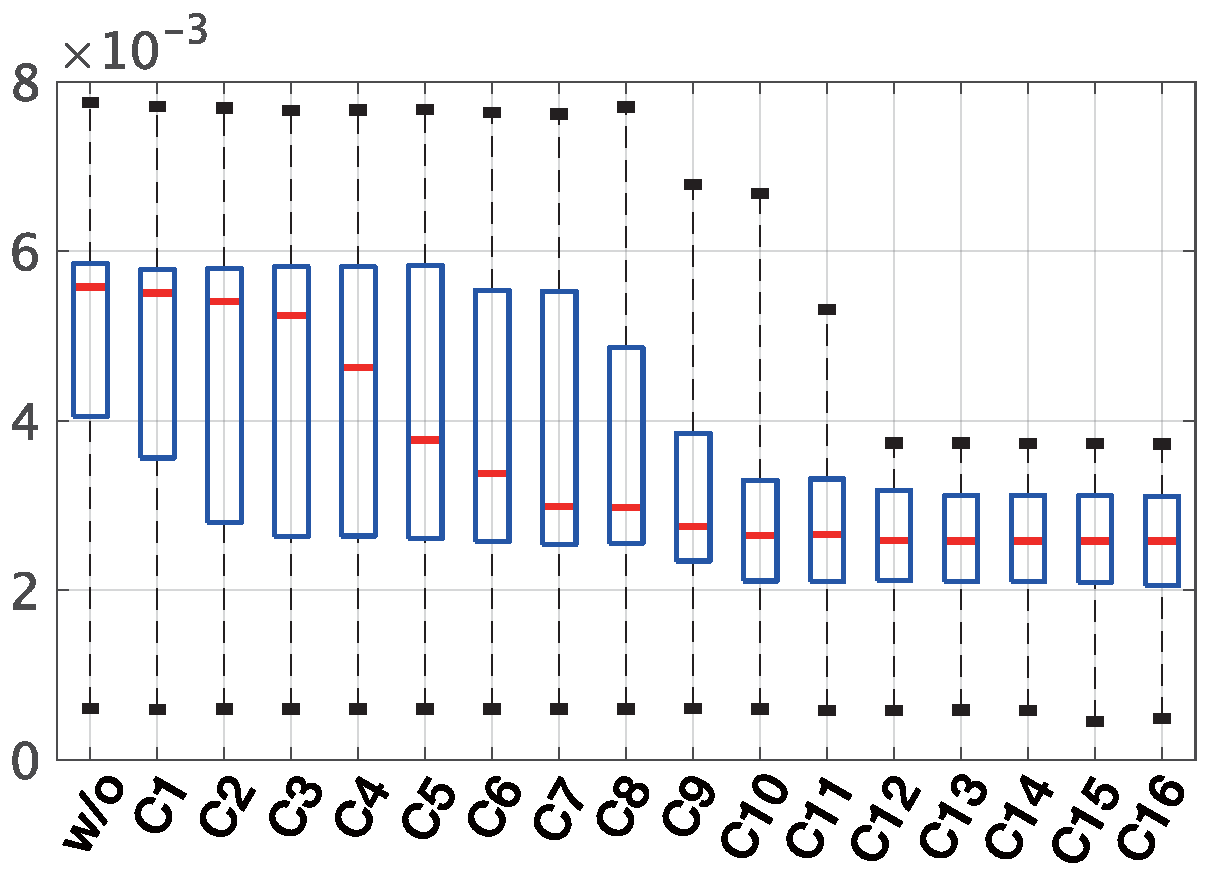
\includegraphics[width = 1.0\linewidth]{figs/boxplotgen}
    \subcaption{ $\mathcal{J}_{\rm G}$: Ground fault on generator buses}
  \end{minipage}
  \begin{minipage}{0.49\linewidth}
    \centering
    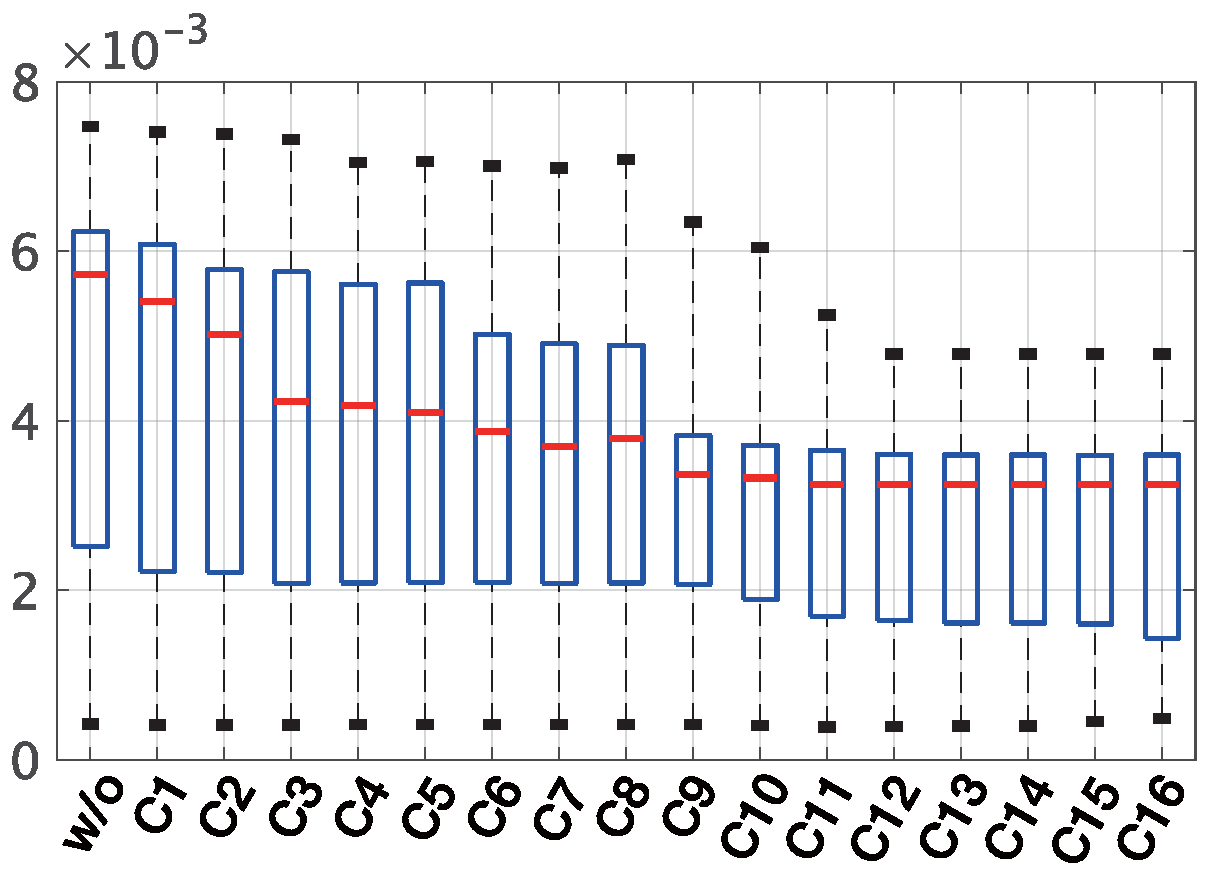
\includegraphics[width = 1.0\linewidth]{figs/boxplotload}
    \subcaption{ $\mathcal{J}_{\rm L}$: Ground fault on load buses}
  \end{minipage}
  \medskip
  \caption{\textbf{Evaluation of system stability with respect to bus ground fault} }
  \label{fig:boxplots}
  }
\medskip
\end{figure}

First, we analyze the transient stability when all generators are equipped with
standard automatic voltage regulators and system stabilizers. The parameter
settings are the same as in Section \ref{sec:onlyAVR}. The results of the
obtained data sets $\mathcal{J}_{\rm G}$ and $\mathcal{J}_{\rm L}$ displayed as
boxplots are shown in the first column of Figure \ref{fig:boxplots}. Figure
\ref{fig:boxplots}(a) shows $\mathcal{J}_{\rm G}$ regarding the ground fault on
the generator bus, and Figure \ref{fig:boxplots}(b) shows $\mathcal{J}_{\rm L}$
regarding the ground fault on the load bus. Subsequently, we evaluate the
improvement of transient stability due to the addition of local controllers
based on these values as a reference.

\subsection{Effect of power system stabilizers bassed on retrofit control theory}

We analyze the transient stability when power system stabilizers based on the
retrofit control theory explained in Section \ref{sec:retrofit} are incorporated
into each generator. The retrofit controllers incorporated into each generator
use the parameters of the approximate linear environment model identified from
measurement data using the procedure described in Example \ref{ex:modelingV}. In
addition to the automatic voltage regulator, the model of the power system
stabilizer is also used in the local linear subsystem $G_i$. Furthermore, the
controller that stabilizes each design model $G_i^+$ is designed based on the
linear quadratic regulator design method explained in Section
\ref{sec:designret}.

In this case, we show the results of displaying the obtained data sets
$\mathcal{J}_{\rm G}$ and $\mathcal{J}_{\rm L}$ as box-and-whisker plots in the
second to seventeenth columns of Figure \ref{fig:boxplots}. The horizontal axis
"C$i$" represents the case where retrofit controllers are incorporated into all
generators from generator 1 to generator $i$. From these results, we can see
that the transient stability gradually improves as the number of retrofit
controllers incorporated increases.

\begin{table}[ht]
\medskip
\caption{\textbf{Physical constants of transmission lines}} \label{table:ieee68lines}
 \centering
  {
  \begin{minipage}{0.49\linewidth}
    \centering
  \begin{tabular}{crrrrcc}
   \hline
$i$--$j$ & $r_{ij}$  &  $x_{ij}$ & $c_{ij}$ \\
   \hline \hline
1--54  & 0 & 0.0181 & 0 \\
2--58  & 0 & 0.0250 & 0 \\
3--62  & 0 & 0.0200 & 0 \\
4--19  & 0.0007 & 0.0142 & 0 \\
5--20  & 0.0009 & 0.0180 & 0 \\
6--22  & 0 & 0.0143 & 0 \\
7--23  & 0.0005 & 0.0272 & 0 \\
8--25  & 0.0006 & 0.0232 & 0 \\
9--29  & 0.0008 & 0.0156 & 0 \\
10--31  & 0 & 0.0260 & 0 \\
11--32  & 0 & 0.0130 & 0 \\
12--36  & 0 & 0.0075 & 0 \\
13--17  & 0 & 0.0033 & 0 \\
14--41  & 0 & 0.0015 & 0 \\
15--42  & 0 & 0.0015 & 0 \\
16--18  & 0 & 0.0030 & 0 \\
17--36  & 0.0005 & 0.0045 & 0.3200 \\
17--43  & 0.0005 & 0.0276 & 0 \\
18--42  & 0.0040 & 0.0600 & 2.2500 \\
18--49  & 0.0076 & 0.1141 & 1.1600 \\
19--20  & 0.0007 & 0.0138 & 0 \\
19--68  & 0.0016 & 0.0195 & 0.3040 \\
21--22  & 0.0008 & 0.0140 & 0.2565 \\
21--68  & 0.0008 & 0.0135 & 0.2548 \\
22--23  & 0.0006 & 0.0096 & 0.1846 \\
23--24  & 0.0022 & 0.0350 & 0.3610 \\
24--68  & 0.0003 & 0.0059 & 0.0680 \\
25--26  & 0.0032 & 0.0323 & 0.5310 \\
25--54  & 0.0070 & 0.0086 & 0.1460 \\
26--27  & 0.0014 & 0.0147 & 0.2396 \\
26--28  & 0.0043 & 0.0474 & 0.7802 \\
26--29  & 0.0057 & 0.0625 & 1.0290 \\
27--37  & 0.0013 & 0.0173 & 0.3216 \\
27--53  & 0.0320 & 0.3200 & 0.4100 \\
28--29  & 0.0014 & 0.0151 & 0.2490 \\
30--31  & 0.0013 & 0.0187 & 0.3330 \\
30--32  & 0.0024 & 0.0288 & 0.4880 \\
30--53  & 0.0008 & 0.0074 & 0.4800 \\
30--61  & 0.0019 & 0.0183 & 0.2900 \\
30--61  & 0.0019 & 0.0183 & 0.2900 \\
31--38  & 0.0011 & 0.0147 & 0.2470 \\
31--53  & 0.0016 & 0.0163 & 0.2500 \\
32--33  & 0.0008 & 0.0099 & 0.1680 \\
\hline
  \end{tabular}
%  \subcaption{データシート}
  \end{minipage}
  \begin{minipage}{0.49\linewidth}
    \centering
  \begin{tabular}{crrrcc}
   \hline
$i$--$j$ & $r_{ij}$  &  $x_{ij}$ & $c_{ij}$ \\
   \hline \hline
33--34  & 0.0011 & 0.0157 & 0.2020 \\
33--38  & 0.0036 & 0.0444 & 0.6930 \\
34--35  & 0.0001 & 0.0074 & 0 \\
34--36  & 0.0033 & 0.0111 & 1.4500 \\
35--45  & 0.0007 & 0.0175 & 1.3900 \\
36--61  & 0.0022 & 0.0196 & 0.3400 \\
36--61  & 0.0022 & 0.0196 & 0.3400 \\
37--52  & 0.0007 & 0.0082 & 0.1319 \\
37--68  & 0.0007 & 0.0089 & 0.1342 \\
38--46  & 0.0022 & 0.0284 & 0.4300 \\
39--44  & 0 & 0.0411 & 0 \\
39--45  & 0 & 0.0839 & 0 \\
40--41  & 0.0060 & 0.0840 & 3.1500 \\
40--48  & 0.0020 & 0.0220 & 1.2800 \\
41--42  & 0.0040 & 0.0600 & 2.2500 \\
43--44  & 0.0001 & 0.0011 & 0 \\
44--45  & 0.0025 & 0.0730 & 0 \\
45--51  & 0.0004 & 0.0105 & 0.7200 \\
46--49  & 0.0018 & 0.0274 & 0.2700 \\
47--48  & 0.0025 & 0.0268 & 0.4000 \\
47--48  & 0.0025 & 0.0268 & 0.4000 \\
47--53  & 0.0013 & 0.0188 & 1.3100 \\
50--51  & 0.0009 & 0.0221 & 1.6200 \\
52--55  & 0.0011 & 0.0133 & 0.2138 \\
53--54  & 0.0035 & 0.0411 & 0.6987 \\
54--55  & 0.0013 & 0.0151 & 0.2572 \\
55--56  & 0.0013 & 0.0213 & 0.2214 \\
56--57  & 0.0008 & 0.0128 & 0.1342 \\
56--66  & 0.0008 & 0.0129 & 0.1382 \\
57--58  & 0.0002 & 0.0026 & 0.0434 \\
58--59  & 0.0006 & 0.0092 & 0.1130 \\
57--60  & 0.0008 & 0.0112 & 0.1476 \\
59--60  & 0.0004 & 0.0046 & 0.0780 \\
60--61  & 0.0023 & 0.0363 & 0.3804 \\
58--63  & 0.0007 & 0.0082 & 0.1389 \\
62--63  & 0.0004 & 0.0043 & 0.0729 \\
62--65  & 0.0004 & 0.0043 & 0.0729 \\
63--64  & 0.0016 & 0.0435 & 0 \\
64--65  & 0.0016 & 0.0435 & 0 \\
65--66  & 0.0009 & 0.0101 & 0.1723 \\
66--67  & 0.0018 & 0.0217 & 0.3660 \\
67--68  & 0.0009 & 0.0094 & 0.1710 \\
\\
   \hline
  \end{tabular}
%   \subcaption{潮流計算結果}
  \end{minipage}
  }
\end{table}


\begin{table}[ht]
\medskip
\caption{\textbf{Physical constants of generators}} \label{table:ieee68genpara}
 \centering
 {
\begin{tabular}{crrrrrr}
   \hline
\multicolumn{1}{c}{$i$} & \multicolumn{1}{r}{$M_{i}$} & \multicolumn{1}{r}{$D_{i}$} & \multicolumn{1}{r}{$\tau_{i}$} & \multicolumn{1}{r}{$X_{{\rm d}i}$} & \multicolumn{1}{r}{$X_{{\rm q}i}$} & \multicolumn{1}{r}{$X_{{\rm d}i}'$}  \\
   \hline \hline
1  & \multicolumn{1}{r}{42.0}  & \multicolumn{1}{r}{4.00} & \multicolumn{1}{r}{10.20} & \multicolumn{1}{r}{0.100} & \multicolumn{1}{r}{0.069} & \multicolumn{1}{r}{0.031} \\
2  & \multicolumn{1}{r}{30.2}  & \multicolumn{1}{r}{9.75} & \multicolumn{1}{r}{6.56} & \multicolumn{1}{r}{0.295} & \multicolumn{1}{r}{0.282} & \multicolumn{1}{r}{0.070} \\
3  & \multicolumn{1}{r}{35.8}  & \multicolumn{1}{r}{10.00} & \multicolumn{1}{r}{5.70} & \multicolumn{1}{r}{0.250} & \multicolumn{1}{r}{0.237} & \multicolumn{1}{r}{0.053} \\
4  & \multicolumn{1}{r}{28.6}  & \multicolumn{1}{r}{10.00} & \multicolumn{1}{r}{5.69} & \multicolumn{1}{r}{0.262} & \multicolumn{1}{r}{0.258} & \multicolumn{1}{r}{0.044} \\
5  & \multicolumn{1}{r}{26.0}  & \multicolumn{1}{r}{3.00} & \multicolumn{1}{r}{5.40} & \multicolumn{1}{r}{0.330} & \multicolumn{1}{r}{0.310} & \multicolumn{1}{r}{0.066} \\
6  & \multicolumn{1}{r}{34.8}  & \multicolumn{1}{r}{10.00} & \multicolumn{1}{r}{7.30} & \multicolumn{1}{r}{0.254} & \multicolumn{1}{r}{0.241} & \multicolumn{1}{r}{0.050} \\
7  & \multicolumn{1}{r}{26.4}  & \multicolumn{1}{r}{8.00} & \multicolumn{1}{r}{5.66} & \multicolumn{1}{r}{0.295} & \multicolumn{1}{r}{0.292} & \multicolumn{1}{r}{0.049} \\
8  & \multicolumn{1}{r}{24.3}  & \multicolumn{1}{r}{9.00} & \multicolumn{1}{r}{6.70} & \multicolumn{1}{r}{0.290} & \multicolumn{1}{r}{0.280} & \multicolumn{1}{r}{0.057} \\
9  & \multicolumn{1}{r}{34.5}  & \multicolumn{1}{r}{14.00} & \multicolumn{1}{r}{4.79} & \multicolumn{1}{r}{0.211} & \multicolumn{1}{r}{0.205} & \multicolumn{1}{r}{0.057} \\
10 & \multicolumn{1}{r}{31.0}  & \multicolumn{1}{r}{5.56} & \multicolumn{1}{r}{9.37} & \multicolumn{1}{r}{0.169} & \multicolumn{1}{r}{0.115} & \multicolumn{1}{r}{0.046} \\
11 & \multicolumn{1}{r}{28.2}  & \multicolumn{1}{r}{13.60} & \multicolumn{1}{r}{4.10} & \multicolumn{1}{r}{0.128} & \multicolumn{1}{r}{0.123} & \multicolumn{1}{r}{0.018} \\
12 & \multicolumn{1}{r}{92.3}  & \multicolumn{1}{r}{13.50} & \multicolumn{1}{r}{7.40} & \multicolumn{1}{r}{0.101} & \multicolumn{1}{r}{0.095} & \multicolumn{1}{r}{0.031} \\
13 & \multicolumn{1}{r}{248.0}  & \multicolumn{1}{r}{33.00} & \multicolumn{1}{r}{5.90} & \multicolumn{1}{r}{0.030} & \multicolumn{1}{r}{0.029} & \multicolumn{1}{r}{0.006} \\
14 & \multicolumn{1}{r}{300.0}  & \multicolumn{1}{r}{100.00} & \multicolumn{1}{r}{4.10} & \multicolumn{1}{r}{0.018} & \multicolumn{1}{r}{0.017} & \multicolumn{1}{r}{0.003} \\
15 & \multicolumn{1}{r}{300.0}  & \multicolumn{1}{r}{100.00} & \multicolumn{1}{r}{4.10} & \multicolumn{1}{r}{0.018} & \multicolumn{1}{r}{0.017} & \multicolumn{1}{r}{0.003} \\
16 & \multicolumn{1}{r}{225.0}  & \multicolumn{1}{r}{50.00} & \multicolumn{1}{r}{7.80} & \multicolumn{1}{r}{0.036} & \multicolumn{1}{r}{0.033} & \multicolumn{1}{r}{0.007} \\
\hline
\end{tabular}
}
\end{table}





\begin{table}[ht]
\medskip
\caption{\textbf{Datasheet for tidal current calculations (generator bus bar)}} \label{table:ieee68datag}
 \centering
  {
  \begin{minipage}{0.32\linewidth}
    \centering
  \begin{tabular}{crrcc}
   \hline
$i$ & $P_i^{\star}$  &  $|\bm{V}_i^{\star} |$ \\
   \hline \hline
1  & \multicolumn{1}{r}{2.50}   & \multicolumn{1}{r}{1.045} \\
2  & \multicolumn{1}{r}{5.45}   & \multicolumn{1}{r}{0.980} \\
3  & \multicolumn{1}{r}{6.50}   & \multicolumn{1}{r}{0.983} \\
4  & \multicolumn{1}{r}{6.32}   & \multicolumn{1}{r}{0.997} \\
5  & \multicolumn{1}{r}{5.05}   & \multicolumn{1}{r}{1.011} \\
6  & \multicolumn{1}{r}{7.00}   & \multicolumn{1}{r}{1.050} \\
   \hline
  \end{tabular}
%  \subcaption{データシート}
  \end{minipage}
  \begin{minipage}{0.32\linewidth}
    \centering
  \begin{tabular}{ccccc}
   \hline
$i$ & $P_i^{\star}$  &  $|\bm{V}_i^{\star} |$ \\
   \hline \hline
7  & \multicolumn{1}{r}{5.60}   & \multicolumn{1}{r}{1.063} \\
8  & \multicolumn{1}{r}{5.40}   & \multicolumn{1}{r}{1.030} \\
9  & \multicolumn{1}{r}{8.00}   & \multicolumn{1}{r}{1.025} \\
10 & \multicolumn{1}{r}{5.00}   & \multicolumn{1}{r}{1.010} \\
11 & \multicolumn{1}{r}{10.00}   & \multicolumn{1}{r}{1.000} \\
12 & \multicolumn{1}{r}{13.50}   & \multicolumn{1}{r}{1.016} \\
   \hline
  \end{tabular}
%   \subcaption{潮流計算結果}
  \end{minipage}
    \begin{minipage}{0.32\linewidth}
    \centering
  \begin{tabular}{ccccc}
   \hline
$i$ & $P_i^{\star}$  &  $|\bm{V}_i^{\star} |$ \\
   \hline \hline
13  & \multicolumn{1}{r}{35.91}   & \multicolumn{1}{r}{1.011} \\
14  & \multicolumn{1}{r}{17.85}   & \multicolumn{1}{r}{1.000} \\
15  & \multicolumn{1}{r}{10.00}   & \multicolumn{1}{r}{1.000} \\
16  & \multicolumn{1}{r}{40.00}   & \multicolumn{1}{r}{1.000} \\
\\
\\
   \hline
  \end{tabular}
%   \subcaption{潮流計算結果}
  \end{minipage}
  }
\end{table}
 
 
\begin{table}[ht]
\medskip
\caption{\textbf{Datasheet used for tidal current calculations (load bus bar)}} \label{table:ieee68datal}
 \centering
  {
  \begin{minipage}{0.32\linewidth}
    \centering
  \begin{tabular}{crrcc}
   \hline
$i$ & $P_i^{\star}$  &  $Q_i^{\star}$ \\
   \hline \hline
\multicolumn{1}{c}{17}  & \multicolumn{1}{r}{$-$60.00} & \multicolumn{1}{r}{$-$3.00} \\
\multicolumn{1}{c}{18}  & \multicolumn{1}{r}{$-$24.70} & \multicolumn{1}{r}{$-$1.23}  \\
\multicolumn{1}{c}{19}  & \multicolumn{1}{r}{0} & \multicolumn{1}{r}{0}  \\
\multicolumn{1}{c}{20}  & \multicolumn{1}{r}{$-$6.80} & \multicolumn{1}{r}{$-$1.03}  \\
\multicolumn{1}{c}{21}  & \multicolumn{1}{r}{$-$2.74} & \multicolumn{1}{r}{$-$1.15}  \\
\multicolumn{1}{c}{22}  & \multicolumn{1}{r}{0} & \multicolumn{1}{r}{0}  \\
\multicolumn{1}{c}{23}  & \multicolumn{1}{r}{$-$2.48} & \multicolumn{1}{r}{$-$0.85} \\
\multicolumn{1}{c}{24}  & \multicolumn{1}{r}{$-$3.09} & \multicolumn{1}{r}{0.92} \\
\multicolumn{1}{c}{25}  & \multicolumn{1}{r}{$-$2.24} & \multicolumn{1}{r}{$-$0.47} \\
\multicolumn{1}{c}{26}  & \multicolumn{1}{r}{$-$1.39} & \multicolumn{1}{r}{$-$0.17}  \\
\multicolumn{1}{c}{27}  & \multicolumn{1}{r}{$-$2.81} & \multicolumn{1}{r}{$-$0.76} \\
\multicolumn{1}{c}{28}  & \multicolumn{1}{r}{$-$2.06} & \multicolumn{1}{r}{$-$0.28}  \\
\multicolumn{1}{c}{29}  & \multicolumn{1}{r}{$-$2.84} & \multicolumn{1}{r}{$-$0.27}  \\
\multicolumn{1}{c}{30}  & \multicolumn{1}{r}{0} & \multicolumn{1}{r}{0} \\
\multicolumn{1}{c}{31}  & \multicolumn{1}{r}{0} & \multicolumn{1}{r}{0} \\
\multicolumn{1}{c}{32}  & \multicolumn{1}{r}{0} & \multicolumn{1}{r}{0} \\
\multicolumn{1}{c}{33}  & \multicolumn{1}{r}{$-$1.12} & \multicolumn{1}{r}{0} \\
\multicolumn{1}{c}{34}  & \multicolumn{1}{r}{0} & \multicolumn{1}{r}{0} \\
   \hline
  \end{tabular}
%  \subcaption{データシート}
  \end{minipage}
  \begin{minipage}{0.32\linewidth}
    \centering
  \begin{tabular}{crrcc}
   \hline
$i$ & $P_i^{\star}$  &  $Q_i^{\star}$ \\
   \hline \hline
\multicolumn{1}{c}{35}  & \multicolumn{1}{r}{0} & \multicolumn{1}{r}{0} \\
\multicolumn{1}{c}{36}  & \multicolumn{1}{r}{$-$1.02} & \multicolumn{1}{r}{0.19} \\
\multicolumn{1}{c}{37}  & \multicolumn{1}{r}{0} & \multicolumn{1}{r}{0} \\
\multicolumn{1}{c}{38}  & \multicolumn{1}{r}{0} & \multicolumn{1}{r}{0} \\
\multicolumn{1}{c}{39}  & \multicolumn{1}{r}{$-$2.67} & \multicolumn{1}{r}{$-$0.13} \\
\multicolumn{1}{c}{40}  & \multicolumn{1}{r}{$-$0.65} & \multicolumn{1}{r}{$-$0.24} \\
\multicolumn{1}{c}{41}  & \multicolumn{1}{r}{$-$10.00} & \multicolumn{1}{r}{$-$2.50} \\
\multicolumn{1}{c}{42}  & \multicolumn{1}{r}{$-$11.50} & \multicolumn{1}{r}{$-$2.50} \\
\multicolumn{1}{c}{43}  & \multicolumn{1}{r}{0} & \multicolumn{1}{r}{0} \\
\multicolumn{1}{c}{44}  & \multicolumn{1}{r}{$-$2.68} & \multicolumn{1}{r}{$-$0.05} \\
\multicolumn{1}{c}{45}  & \multicolumn{1}{r}{$-$2.08} & \multicolumn{1}{r}{$-$0.21} \\
\multicolumn{1}{c}{46}  & \multicolumn{1}{r}{$-$1.51} & \multicolumn{1}{r}{$-$0.29} \\
\multicolumn{1}{c}{47}  & \multicolumn{1}{r}{$-$2.03} & \multicolumn{1}{r}{$-$0.33} \\
\multicolumn{1}{c}{48}  & \multicolumn{1}{r}{$-$2.41} & \multicolumn{1}{r}{$-$0.02} \\
\multicolumn{1}{c}{49}  & \multicolumn{1}{r}{$-$1.64} & \multicolumn{1}{r}{$-$0.29} \\
\multicolumn{1}{c}{50}  & \multicolumn{1}{r}{$-$1.00} & \multicolumn{1}{r}{1.47} \\
\multicolumn{1}{c}{51}  & \multicolumn{1}{r}{$-$3.37} & \multicolumn{1}{r}{1.22} \\
\multicolumn{1}{c}{52}  & \multicolumn{1}{r}{$-$1.58} & \multicolumn{1}{r}{$-$0.30} \\
   \hline
  \end{tabular}
%   \subcaption{潮流計算結果}
  \end{minipage}
    \begin{minipage}{0.32\linewidth}
    \centering
  \begin{tabular}{crrcc}
   \hline
$i$ & $P_i^{\star}$  &  $Q_i^{\star}$ \\
   \hline \hline
\multicolumn{1}{c}{53}  & \multicolumn{1}{r}{$-$2.52} & \multicolumn{1}{r}{$-$1.19} \\
\multicolumn{1}{c}{54}  & \multicolumn{1}{r}{0} & \multicolumn{1}{r}{0} \\
\multicolumn{1}{c}{55}  & \multicolumn{1}{r}{$-$3.22} & \multicolumn{1}{r}{$-$0.02} \\
\multicolumn{1}{c}{56}  & \multicolumn{1}{r}{$-$2.00} & \multicolumn{1}{r}{$-$0.74} \\
\multicolumn{1}{c}{57}  & \multicolumn{1}{r}{0} & \multicolumn{1}{r}{0} \\
\multicolumn{1}{c}{58}  & \multicolumn{1}{r}{0} & \multicolumn{1}{r}{0} \\
\multicolumn{1}{c}{59}  & \multicolumn{1}{r}{$-$2.34} & \multicolumn{1}{r}{$-$0.84} \\
\multicolumn{1}{c}{60}  & \multicolumn{1}{r}{$-$2.09} & \multicolumn{1}{r}{$-$0.71} \\
\multicolumn{1}{c}{61}  & \multicolumn{1}{r}{$-$1.04} & \multicolumn{1}{r}{$-$1.25} \\
\multicolumn{1}{c}{62}  & \multicolumn{1}{r}{0} & \multicolumn{1}{r}{0} \\
\multicolumn{1}{c}{63}  & \multicolumn{1}{r}{0} & \multicolumn{1}{r}{0} \\
\multicolumn{1}{c}{64}  & \multicolumn{1}{r}{$-$0.09} & \multicolumn{1}{r}{$-$0.88} \\
\multicolumn{1}{c}{65}  & \multicolumn{1}{r}{0} & \multicolumn{1}{r}{0} \\
\multicolumn{1}{c}{66}  & \multicolumn{1}{r}{0} & \multicolumn{1}{r}{0} \\
\multicolumn{1}{c}{67}  & \multicolumn{1}{r}{$-$3.20} & \multicolumn{1}{r}{$-$1.53} \\
\multicolumn{1}{c}{68}  & \multicolumn{1}{r}{$-$3.29} & \multicolumn{1}{r}{$-$0.32} \\
\\
\\
   \hline
  \end{tabular}
%   \subcaption{潮流計算結果}
  \end{minipage}
  }
\end{table}







\begin{table}[ht]
\medskip
\caption{\textbf{Load impedance}} \label{table:ieee68loads}
 \centering
  {
  \begin{minipage}{0.32\linewidth}
    \centering
  \begin{tabular}{crrcc}
   \hline
$i$ & $r_{{\rm load}i}$  &  $x_{{\rm load}i}$ \\
   \hline \hline
\multicolumn{1}{c}{17}  & \multicolumn{1}{r}{$-$60.00} & \multicolumn{1}{r}{$-$3.00} \\
\multicolumn{1}{c}{18}  & \multicolumn{1}{r}{$-$24.70} & \multicolumn{1}{r}{$-$1.23}  \\
\multicolumn{1}{c}{19}  & \multicolumn{1}{r}{0} & \multicolumn{1}{r}{0}  \\
\multicolumn{1}{c}{20}  & \multicolumn{1}{r}{$-$6.80} & \multicolumn{1}{r}{$-$1.03}  \\
\multicolumn{1}{c}{21}  & \multicolumn{1}{r}{$-$2.74} & \multicolumn{1}{r}{$-$1.15}  \\
\multicolumn{1}{c}{22}  & \multicolumn{1}{r}{0} & \multicolumn{1}{r}{0}  \\
\multicolumn{1}{c}{23}  & \multicolumn{1}{r}{$-$2.48} & \multicolumn{1}{r}{$-$0.85} \\
\multicolumn{1}{c}{24}  & \multicolumn{1}{r}{$-$3.09} & \multicolumn{1}{r}{0.92} \\
\multicolumn{1}{c}{25}  & \multicolumn{1}{r}{$-$2.24} & \multicolumn{1}{r}{$-$0.47} \\
\multicolumn{1}{c}{26}  & \multicolumn{1}{r}{$-$1.39} & \multicolumn{1}{r}{$-$0.17}  \\
\multicolumn{1}{c}{27}  & \multicolumn{1}{r}{$-$2.81} & \multicolumn{1}{r}{$-$0.76} \\
\multicolumn{1}{c}{28}  & \multicolumn{1}{r}{$-$2.06} & \multicolumn{1}{r}{$-$0.28}  \\
\multicolumn{1}{c}{29}  & \multicolumn{1}{r}{$-$2.84} & \multicolumn{1}{r}{$-$0.27}  \\
\multicolumn{1}{c}{30}  & \multicolumn{1}{r}{0} & \multicolumn{1}{r}{0} \\
\multicolumn{1}{c}{31}  & \multicolumn{1}{r}{0} & \multicolumn{1}{r}{0} \\
\multicolumn{1}{c}{32}  & \multicolumn{1}{r}{0} & \multicolumn{1}{r}{0} \\
\multicolumn{1}{c}{33}  & \multicolumn{1}{r}{$-$1.12} & \multicolumn{1}{r}{0} \\
\multicolumn{1}{c}{34}  & \multicolumn{1}{r}{0} & \multicolumn{1}{r}{0} \\
   \hline
  \end{tabular}
%  \subcaption{データシート}
  \end{minipage}
  \begin{minipage}{0.32\linewidth}
    \centering
  \begin{tabular}{crrcc}
   \hline
$i$ & $r_{{\rm load}i}$  &  $x_{{\rm load}i}$ \\
   \hline \hline
\multicolumn{1}{c}{35}  & \multicolumn{1}{r}{0} & \multicolumn{1}{r}{0} \\
\multicolumn{1}{c}{36}  & \multicolumn{1}{r}{$-$1.02} & \multicolumn{1}{r}{0.19} \\
\multicolumn{1}{c}{37}  & \multicolumn{1}{r}{0} & \multicolumn{1}{r}{0} \\
\multicolumn{1}{c}{38}  & \multicolumn{1}{r}{0} & \multicolumn{1}{r}{0} \\
\multicolumn{1}{c}{39}  & \multicolumn{1}{r}{$-$2.67} & \multicolumn{1}{r}{$-$0.13} \\
\multicolumn{1}{c}{40}  & \multicolumn{1}{r}{$-$0.65} & \multicolumn{1}{r}{$-$0.24} \\
\multicolumn{1}{c}{41}  & \multicolumn{1}{r}{$-$10.00} & \multicolumn{1}{r}{$-$2.50} \\
\multicolumn{1}{c}{42}  & \multicolumn{1}{r}{$-$11.50} & \multicolumn{1}{r}{$-$2.50} \\
\multicolumn{1}{c}{43}  & \multicolumn{1}{r}{0} & \multicolumn{1}{r}{0} \\
\multicolumn{1}{c}{44}  & \multicolumn{1}{r}{$-$2.68} & \multicolumn{1}{r}{$-$0.05} \\
\multicolumn{1}{c}{45}  & \multicolumn{1}{r}{$-$2.08} & \multicolumn{1}{r}{$-$0.21} \\
\multicolumn{1}{c}{46}  & \multicolumn{1}{r}{$-$1.51} & \multicolumn{1}{r}{$-$0.29} \\
\multicolumn{1}{c}{47}  & \multicolumn{1}{r}{$-$2.03} & \multicolumn{1}{r}{$-$0.33} \\
\multicolumn{1}{c}{48}  & \multicolumn{1}{r}{$-$2.41} & \multicolumn{1}{r}{$-$0.02} \\
\multicolumn{1}{c}{49}  & \multicolumn{1}{r}{$-$1.64} & \multicolumn{1}{r}{$-$0.29} \\
\multicolumn{1}{c}{50}  & \multicolumn{1}{r}{$-$1.00} & \multicolumn{1}{r}{1.47} \\
\multicolumn{1}{c}{51}  & \multicolumn{1}{r}{$-$3.37} & \multicolumn{1}{r}{1.22} \\
\multicolumn{1}{c}{52}  & \multicolumn{1}{r}{$-$1.58} & \multicolumn{1}{r}{$-$0.30} \\
   \hline
  \end{tabular}
%   \subcaption{潮流計算結果}
  \end{minipage}
    \begin{minipage}{0.32\linewidth}
    \centering
  \begin{tabular}{crrcc}
   \hline
$i$ & $r_{{\rm load}i}$  &  $x_{{\rm load}i}$ \\
   \hline \hline
\multicolumn{1}{c}{53}  & \multicolumn{1}{r}{$-$2.52} & \multicolumn{1}{r}{$-$1.19} \\
\multicolumn{1}{c}{54}  & \multicolumn{1}{r}{0} & \multicolumn{1}{r}{0} \\
\multicolumn{1}{c}{55}  & \multicolumn{1}{r}{$-$3.22} & \multicolumn{1}{r}{$-$0.02} \\
\multicolumn{1}{c}{56}  & \multicolumn{1}{r}{$-$2.00} & \multicolumn{1}{r}{$-$0.74} \\
\multicolumn{1}{c}{57}  & \multicolumn{1}{r}{0} & \multicolumn{1}{r}{0} \\
\multicolumn{1}{c}{58}  & \multicolumn{1}{r}{0} & \multicolumn{1}{r}{0} \\
\multicolumn{1}{c}{59}  & \multicolumn{1}{r}{$-$2.34} & \multicolumn{1}{r}{$-$0.84} \\
\multicolumn{1}{c}{60}  & \multicolumn{1}{r}{$-$2.09} & \multicolumn{1}{r}{$-$0.71} \\
\multicolumn{1}{c}{61}  & \multicolumn{1}{r}{$-$1.04} & \multicolumn{1}{r}{$-$1.25} \\
\multicolumn{1}{c}{62}  & \multicolumn{1}{r}{0} & \multicolumn{1}{r}{0} \\
\multicolumn{1}{c}{63}  & \multicolumn{1}{r}{0} & \multicolumn{1}{r}{0} \\
\multicolumn{1}{c}{64}  & \multicolumn{1}{r}{$-$0.09} & \multicolumn{1}{r}{$-$0.88} \\
\multicolumn{1}{c}{65}  & \multicolumn{1}{r}{0} & \multicolumn{1}{r}{0} \\
\multicolumn{1}{c}{66}  & \multicolumn{1}{r}{0} & \multicolumn{1}{r}{0} \\
\multicolumn{1}{c}{67}  & \multicolumn{1}{r}{$-$3.20} & \multicolumn{1}{r}{$-$1.53} \\
\multicolumn{1}{c}{68}  & \multicolumn{1}{r}{$-$3.29} & \multicolumn{1}{r}{$-$0.32} \\
\\
\\
   \hline
  \end{tabular}
%   \subcaption{潮流計算結果}
  \end{minipage}
  }
\end{table}


\newpage
%\printindex
%
%
\end{document}